\documentclass[11pt, letterpaper]{article}
\usepackage{cite}
\usepackage{amsmath}
\usepackage{mathtools}
\usepackage[numbers,sort&compress]{natbib}
\UseRawInputEncoding
%\usepackage[T1]{fontenc}
%\usepackage[utf8]{inputenc}
\usepackage[margin=1in,letterpaper]{geometry}
\usepackage{ragged2e,setspace,graphicx,lipsum,xcolor,titling,float,titlesec,subcaption,expex}
\usepackage{marvosym,tabularray}
\usepackage{xurl}

\usepackage{tipa}
%\DeclareFontSubstitution{T3}{ptm}{el}{n}
\graphicspath{ {figures/} }
\linespread{1} %1 = single, 1.3= 1.5 spacing, 1.6 = double

\usepackage{times}
\frenchspacing

%\let\Cross\relax
%\usepackage{bbding}

%headers 
\usepackage{fancyhdr}
\setlength{\headheight}{13.6pt} % needs to be above 13.6 to work right
\pagestyle{fancy}
\newcommand{\changefont}{ \fontsize{9}{11} \sffamily \selectfont}
\fancyhead{}
\fancyhead[L]{\changefont \textit{Learning \& Story}, \today}
\fancyhead[R]{\changefont CS6000 Computer Science Research}
 
\usepackage{multicol}
\setlength{\columnsep}{0cm}

% defines "abstract" environment
\renewenvironment{abstract}{%
\noindent\begin{minipage}{1\textwidth}
\setlength{\leftskip}{0.38in}
\setlength{\rightskip}{0.38in}}
{\end{minipage}}

% define keyword
\newcommand{\keyword}{\vskip 6pt \par \small \itshape Keywords: }

% define header environment
\renewenvironment{top}{%
\noindent\begin{minipage}{1\textwidth}
\setlength{\leftskip}{0in}
\setlength{\rightskip}{0in}}
{\end{minipage}}

% caption formatting
\captionsetup[figure]{font={sf, small} }
\captionsetup[table]{font={sf, small} }

% section headings
\titleformat*{\section}{\normalsize \sffamily \bfseries}
\titleformat*{\subsection}{\normalsize \sffamily}
\titleformat*{\subsubsection}{\normalsize  \sffamily  \itshape}
\titleformat*{\paragraph}{\normalsize \bfseries}
\titleformat*{\subparagraph}{\normalsize \bfseries}

%{indent}{linebefore}{lineafter} 
%need stars to surpress "indent first line"
\titlespacing*{\section}{0pt}{12pt}{6pt}
\titlespacing*{\section}{0pt}{12pt}{6pt}
\titlespacing*{\subsection}{0pt}{12pt}{6pt}
\titlespacing*{\subsubsection}{0pt}{12pt}{6pt}

%title page and author info
\pretitle{
\vskip 20pt 
\raggedleft
\huge 
\sffamily}
\posttitle{}
\preauthor{
\vskip 17pt
\raggedleft
\large 
\sffamily}
\postauthor{}
\predate{
\vskip 5pt
\raggedleft
\small 
\sffamily}
\postdate{
\small 
\sffamily}

\newcommand{\affiliation}[1]{\date{#1}}
\newcommand{\email}[1] {\href{mailto:#1}{#1}}
  
% how close is it to the top?
\setlength{\droptitle}{-30pt}

%hyperref is a very nasty package, be sure to load it last
\usepackage{hyperref}
\hypersetup{colorlinks = true, urlcolor=blue, filecolor=blue, citecolor = black,linkcolor=black}

\begin{document}
\pagenumbering{arabic}

\title{Learning \& Story}
\author{H. M. A. Mohit Chowdhury}
\affiliation{
\sffamily University of Colorado at Colorado Springs -- \email{hchowdhu@uccs.edu}
}

{\let\newpage\relax\maketitle}

\section{Learning}
There are lots of survey or review papers\cite{yoo_deep_2015,taheri-garavand_meat_2019,brunetti_computer_2018,patricio_computer_2018,li_review_2020,colyer_review_2018,oudah_hand_2020,fang_computer_2020,akhtar_threat_2018,al-kaff_survey_2018,voulodimos_deep_2018,huang_multi-view_2019,feng_computer_2019,buhrmester_analysis_2021,gowrisankaran_computer_2015,dong_review_2021,capitan-vallvey_recent_2015,wang_generative_2021,al-saffar_review_2017,bashar_survey_2019,ioannidou_deep_2017,liu_survey_2018,liu_survey_2017,nguyen_deep_2022,khamparia_systematic_2019,ribaric_-identification_2016,feng_computer_2018,dargan_survey_2020,koch_review_2015,adjabi_past_2020,bayoudh_survey_2022,ye_review_2016,martineau_survey_2017,mehta_facial_2018,bhargava_fruits_2021,corneanu_survey_2016,xu_review_2018,kasar_face_2016,mohan_crack_2018,zhu_handcrafted_2016,hassannejad_automatic_2017,herath_going_2017,lee_deep_2017,jing_self-supervised_2020,yanase_systematic_2019,baqersad_photogrammetry_2017,khan_survey_2020,shanthamallu_brief_2017,cheng_fashion_2021,jain_50_2016,ko_brief_2018,atitallah_leveraging_2020,ota_deep_2017,baltrusaitis_multimodal_2018,dantcheva_what_2015,sundararajan_deep_2018,huang_machine_2018,csapo_survey_2015,wiley_computer_2018,kanellakis_survey_2017,chouhan_applications_2020,khan_machine_2021,guo_attention_2022,le_deep_2021,sampath_survey_2021,akbari_applications_2021,wang_survey_2016,okinda_review_2020,klamm_computer_2015,park_review_2021,tripathi_role_2020,seifert_visualizations_2017,gupta_salient_2020,lukinac_computer_2019,ham_computer_2019,janai_computer_2020,zareiforoush_potential_2015,nyalala_weight_2021,leo_analysis_2020,georgiou_survey_2020,cazzato_survey_2020,chen_survey_2020,rasheed_fabric_2020,sikdar_computer-vision-guided_2016,ekanayake_computer_2021,ahuja_survey_2017,yang_computer_2021,al-faris_review_2020,velesaca_computer_2021,mery_x-ray_2020,gao_computer_2018,shekhar_survey_2020,gazzah_survey_2020,ouhami_computer_2021,thyagharajan_review_2021,lukinac_application_2018,silva_future_2021,zahoor_breast_2020,louis_review_2021,yogameena_computer_2017,an_application_2021,kumar_automatic_2015,santra_comprehensive_2019,di_rosa_fusion_2017,xu_computer_2019,usman_computer_2017,qiu_review_2020,witus_review_2018,junior_first_2018,kour_computer-vision_2019,bhargava_novel_2021,han_survey_2022,bambach_survey_2015,broome_going_2022,jiao_graph_2022,chopde_developments_2017,bv_computer_2018,seo_computer_2015,huttunen_computer_2015,deeb_interreflections_2018,gallego_event-based_2020,velez_embedded_2015,khan_transformers_2021,manchanda_analysis_2016,alhasan_magnitude_2022,ranasinghe_computer_2016,tan_benchmarking_2015,spencer_jr_advances_2019,fernandes_image_2020,liu_deep_2020,zafeiriou_survey_2015,pisharady_recent_2015,de_souza_alves_knowledge_2018,wu_application_2017,singh_review_2020,loce_computer_2017,patel_comprehensive_2020,khan_guide_2018,fortun_optical_2015,gou_knowledge_2021,borji_negative_2018,kong_human_2022,wei-qiang_survey_2022,schneider_past_2019,luo_convolutional_2018,fedorov_detecting_2021,krig_interest_2016,wu_visual_2017,beddiar_vision-based_2020,grys_machine_2017,liu_applications_2021,lyons_deep_2022,belmonte_computer_2019,aloysius_review_2017,wang_rgb-d-based_2018,al_rashidi_computer_2017,hopkins_virtual_2022,watson_virtual_2022,ritchie_computer_2016,dandois_optimal_2015,koohzadi_survey_2017,park_analysis_2020,chouhan_leaf_2021,carballo_new_2019,suryatali_computer_2015,goni_color_2017,sarrafi_comparison_2017,nguyen_computer_2018,kim_using_2018,fang_computer_2018,hirakawa_survey_2018,khan_one_2021,vocaturo_features_2018,zhang_measurement_2021,ji_-field_2021,xu_deep_2019,betancourt_evolution_2015,elsayed_adversarial_2018,borkman_unity_2021} on computer vision and its related topics which helped me a lot to get to know about the use cases of computer vision related topic when I scanned some of them and dive deep with a few of them. Good organization is one of the most important key points for a survey paper where I will target a particular group of people to explore more and attract others to scan at least. A Survey paper should contain some analysis and experimental results which depicts the comparison of the available methods. These experiments should be with different publicly available datasets and with the same methods. Having some graphical representation is another important factor in a good survey paper. Overviewing available methods on a specific topic step by step which seems like a story will increase the readability or the storyline should represent new insight of an existing survey where writer(s) have an interest circulating to others.\\

\section{Adversarial Attacks}
Adversarial attacks is a concern developing computer vision based algorithm while changing a single data can through away the whole system. There are many attacks in computer vision algorithms, especially in DNN and many more are unknown. Pointing out the available attacks and their subsequent results and a hypothesis of some unknown attacks that could be derived from the existing ones will be a safety margin for developing new algorithms and existing ones could be refined. Comparing and contrasting algorithms with different types of data is one of the major challenges. Some algorithms require an array of extensive hardware could be a negative factor hindering others to perform experiments or possibly return from the way as well as me. Comparing both black-box and white-box in all algorithms causes some difficulties and

\begin{figure}[H] \center
    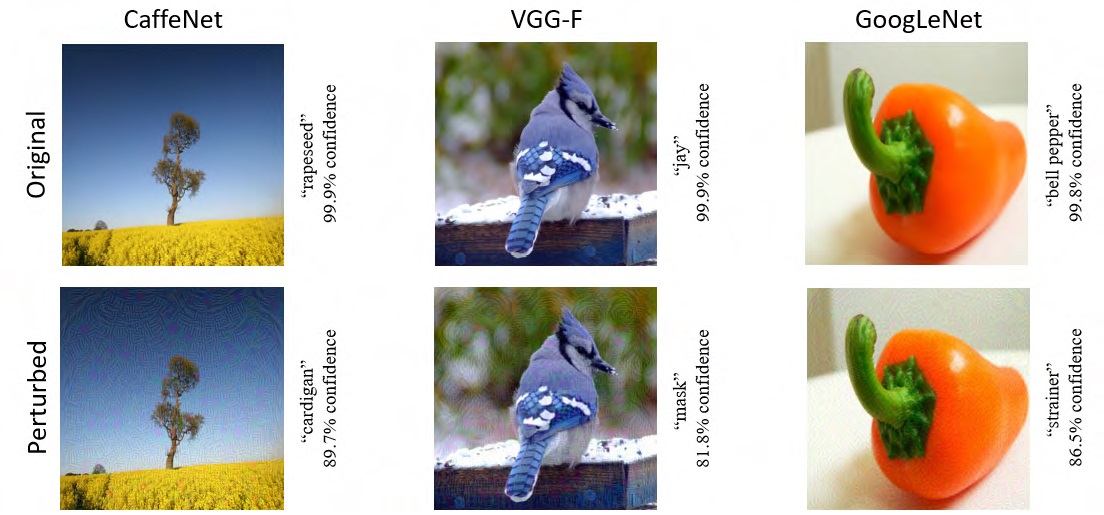
\includegraphics[scale=.5]{./figures/story-1-1.jpg}
    \caption{Adversarial attacks reduce the goal\cite{akhtar_threat_2018}}
    \label{fig:goal-reduction}
\end{figure}\

\begin{figure}[H] \center
\begin{subfigure}{.5\textwidth}
  \centering
  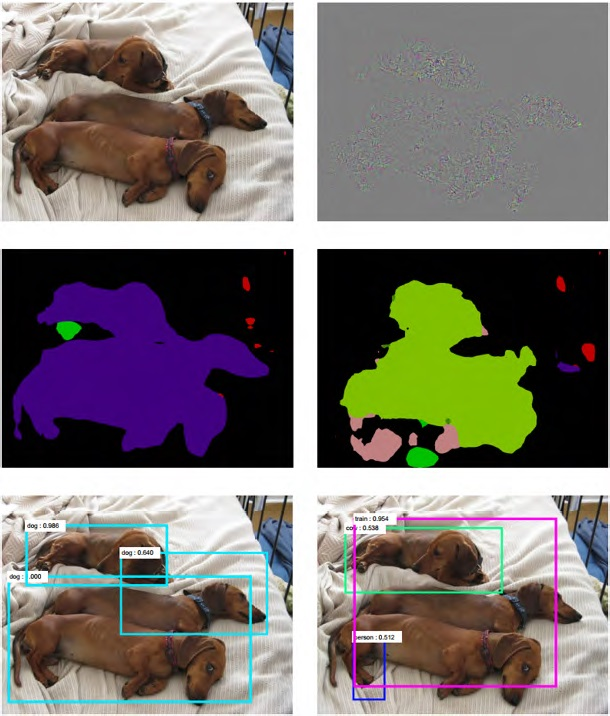
\includegraphics[width=.8\linewidth]{./figures/story-1-2.jpg}
  \caption{Semantic segmentation and object detection flaws due to adversarial attack}
  \label{fig:segmentation-object}
\end{subfigure}%
\begin{subfigure}{.5\textwidth}
  \centering
  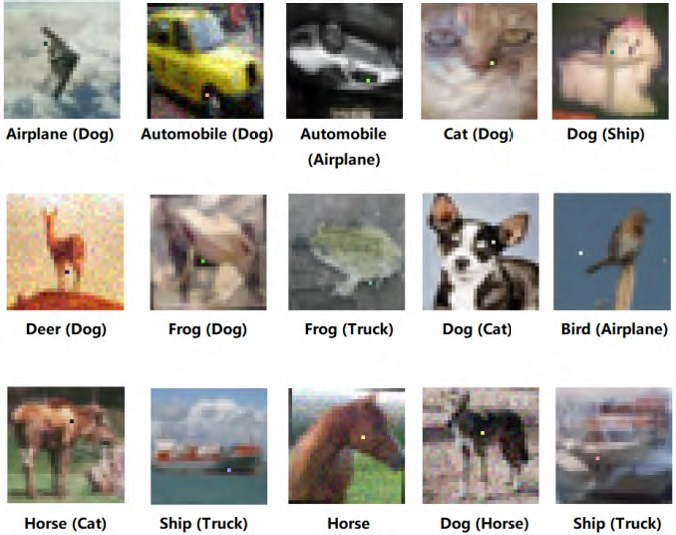
\includegraphics[width=.8\linewidth]{./figures/story-1-3.jpg}
  \caption{One pixel adversarial attack result}
  \label{fig:one-pixel-attack}
\end{subfigure}%
\caption{Experimental result from adversarial attacks\cite{akhtar_threat_2018}}
\label{fig:experimental-results}
\end{figure}

there is no generalized dataset for all the methods. Graphical representation is a way of presenting comparisons or results helping others to get a quick view of attacks pron algorithms encourage a deep dive into finding the gap. In Figure \ref{fig:goal-reduction}, it shows the reduced goal achievement caused by adversarial attacks on different algorithms and the real scenario is depicted in Figure \ref{fig:experimental-results}. There are lots of new methods that should be pointed out with possible attacks. If we could not focus on a specific topic-based algorithm and mess with some old-fashioned algorithms or if there is a lack of important information, possibly we will toward an unsuccessful attempt. Discussing the adversarial attacks vs algorithms, one can find a good picture of all algorithms and its flaws which will help to secure his/her future work or attacker can think about new way of attack. Due to lack of taxonomy and experimental contrast, it may not achieve its audience which is a drawback.\\

\subsection{Story Line}
\begin{itemize}
    \item \textbf{Character}: Adversarial attacks in computer vision algorithms.
    \item \textbf{Character Traits}: Algorithms that can be perturbed with adversarial attacks will draw the attentions.
    \item \textbf{Goal}: Analyzing an algorithm with available datasets and contrasting the benchmark.
    \item \textbf{Motive}: Security of computer vision algorithms.
    \item \textbf{Conflicts/Problems}: From the existing survey, introduction of a new insight and new algorithms vulnerability.
    \item \textbf{Risk/Danger}: If the new algorithms can not be experimented and contrasted with the datasets and lack of essential information and organization.
    \item \textbf{Struggle}: Understanding the algorithms and their implementation and finding out the flaws.
    \item \textbf{Details}: Experimenting with all datasets for an algorithms and making it critical to reach a decision.
\end{itemize}

\section{Markerless Motion Analysis}
Motion analysis and markerless computer vision algorithms are changing the way of our daily life from mobile phones, smart devices, and entertainment to autonomous vehicles, and day by day it is booming. If we take about digital security like a human that can analyze motion and detect unusual movements, computer vision algorithms play the role. There are lots of algorithms for motion analysis and markerless algorithms have their use cases. All of them have their advantages and disadvantage according to specific use cases. Selecting an algorithm for a particular development may be hard to find and algorithms can be used for
\begin{figure}[H] \center
\begin{subfigure}{.5\textwidth}
  \centering
  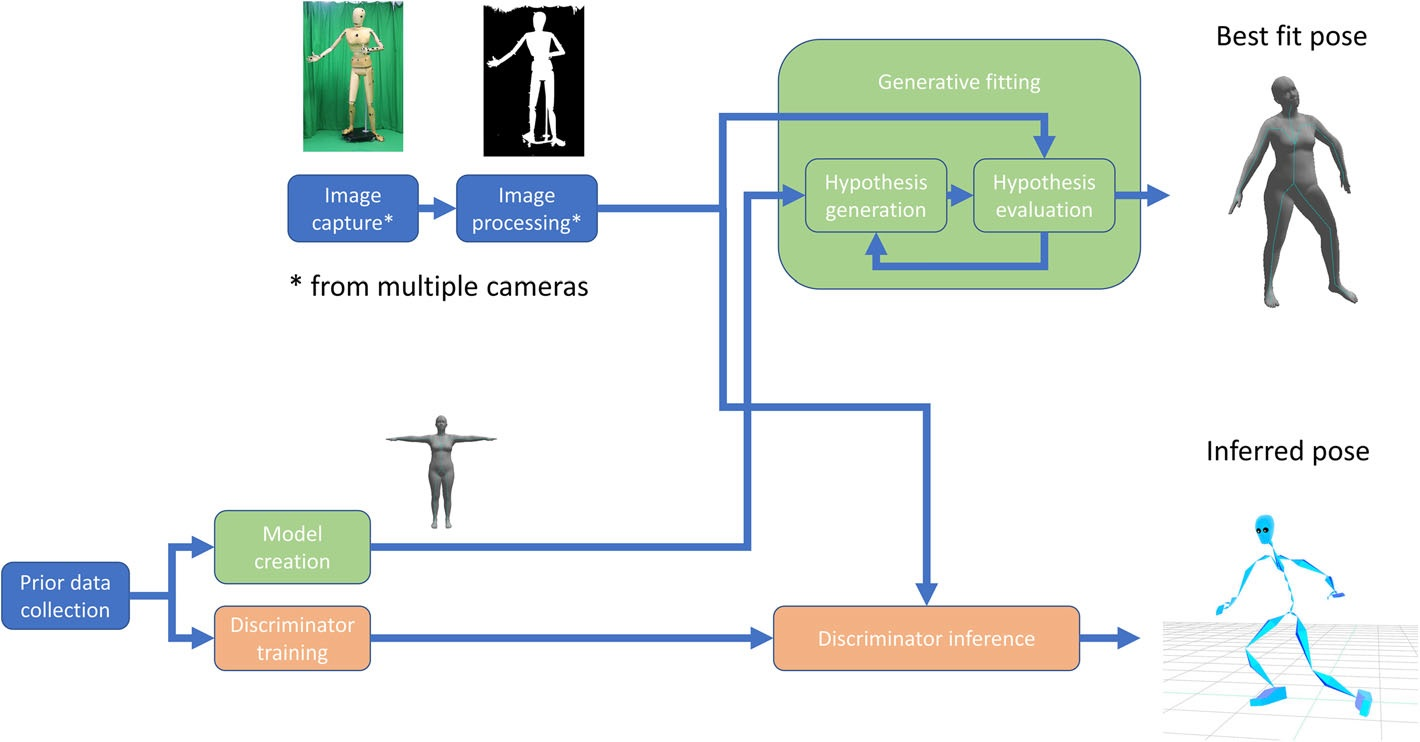
\includegraphics[width=.8\linewidth]{./figures/story-2-1.jpg}
  \caption{Markerless motion general algorithmic overview}
  \label{fig:algo-overview}
\end{subfigure}%
\begin{subfigure}{.5\textwidth}
  \centering
  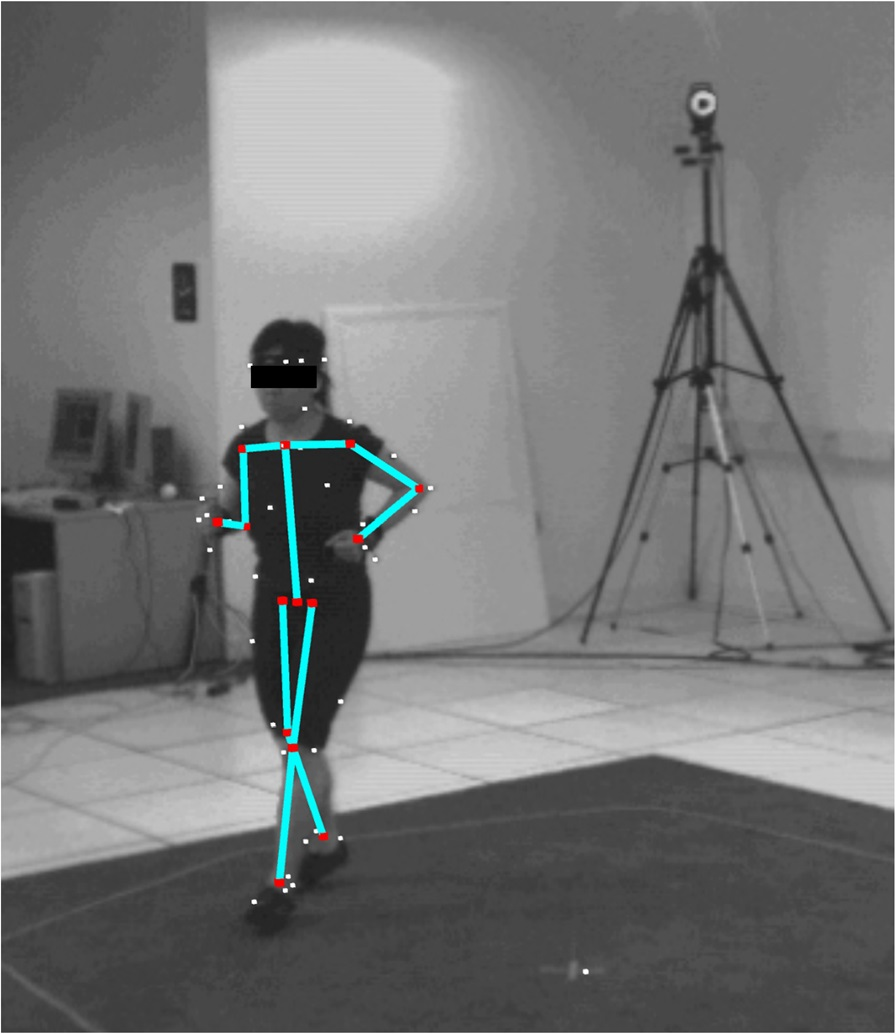
\includegraphics[width=.8\linewidth]{./figures/story-2-2.jpg}
  \caption{An example of motion detection on HumanEva}
  \label{fig:motion-example}
\end{subfigure}%
\caption{Markerless motion detection\cite{colyer_review_2018}}
\label{fig:experimental-results}
\end{figure}
 multiple purposes. Here, we are presenting a one-page review that will help to get a good insight into the whole topic and reveal some new use cases which will be of great value for kick-starting and future research. Figure \ref{fig:algo-overview} depicts a basic methodology of generative and discriminative algorithm for markerless motion detection where the cyan line in Figure\ref{fig:experimental-results} represents the skeleton using the HumanEva dataset. Finding all the tools in one place from different sources and analyzing them with own experiments is a critical process to achieve the goal and there may be a lack of information flow. Arranging publicly available datasets and experiments with a method with all of them is a time-consuming and intensive process. Presenting only the process without analysis and comparison creates a deficiency of a survey and this is one of the risks to catching an eye.\\

\subsection{Story Line}
\begin{itemize}
    \item \textbf{Character}: Markerless motion analysis with computer vision algorithms.
    \item \textbf{Traits}: Bringing all the algorithms in a screen, audience can pick desired one and a brief experimental results will help to compare with each other. 
    \item \textbf{Goal}: Mathematical analysis with publicly available datasets and suggesting real usecases.
    \item \textbf{Motive}: Most of the digital devices make life easy and computer vision is one step ahead of the success.
    \item \textbf{Conflicts/Problems}: Experimenting with all datasets make some hurdle and it needs some tuning. 
    \item \textbf{Risk/Danger}: Without proper analysis with new and old ones and lake of good organization will make it useless at the end.
    \item \textbf{Struggle}: Finding available algorithms and experimenting with real data.
    \item \textbf{Details}: While analyzing with new algorithms, the result was not expected for all data and sometimes it was frustrating.
\end{itemize}

\section{Source}
This journal source is publicly available \href{https://github.com/shadhinaust/cs6000-w4-j4.git}{here}.\\
\bibliographystyle{IEEEtran}
\bibliography{main}
\end{document}
